%%% Article: Software System for Data Acquisition and Analysis Operating the ATLAS-TPX Network
%%% Authors: Petr Manek, Jakub Begera
%%% Copyright (c) 2017 IEAP CTU


\section{\label{sec:analysis}Data Analysis Subsystem}
The Data Analysis Subsystem is comprised of virtual machines hosted at the CERN Meyrin data center and managed by the OpenStack private cloud. Each machine provides a multitude of \textit{worker nodes} responsible for parallel execution of queued \textit{jobs} -- mutually independent operations that interact with data files, providing:
~
\begin{itemize}
  \item Cluster analysis -- morphological classification, converter region determination~\cite{Holy2008}, optionally integration with energy calibration~\cite{Jakubek2011}.
  \item Storage format conversions -- from ASCII plain text to ROOT~\cite{ROOT} and vice versa.
  \item Data consistency verification.
  \item Frame quality checks -- Monte Carlo sampling, alerts are generated when frames violate pre-defined quality criteria.
  \item File transfers -- gzip compression and subsequent archive transfers between Control PC in USA15, EOS and Prague storage infrastructure.
\end{itemize}

Scheduling and completion of such jobs as well as the heartbeat and load state of worker nodes is continuously tracked by a single centralized \textit{manager node}, which indirectly communicates with all workers through shared PostgreSQL database cluster. The cluster operates independently of all nodes, providing additional level of robustness to the entire system. It is responsible for maintaining a priority queue for scheduled jobs, a job locking mechanism for worker nodes, periodically updated worker node manifest and alert delivery system. The underlying database middleware ensures appropriate caching, replication, data persistency and transaction ordering control.

The primary purpose of the Data Analysis Subsystem is to provide reliable infrastructure for automated data verification and evaluation. For reasons of stability and security, these tasks are performed asynchronously with respect to each other and incoming data transfers. In addition to processing new frames, this approach also allows data files to be reprocessed when novel analysis algorithms are introduced.

\begin{figure}[tbp]
  \centering
  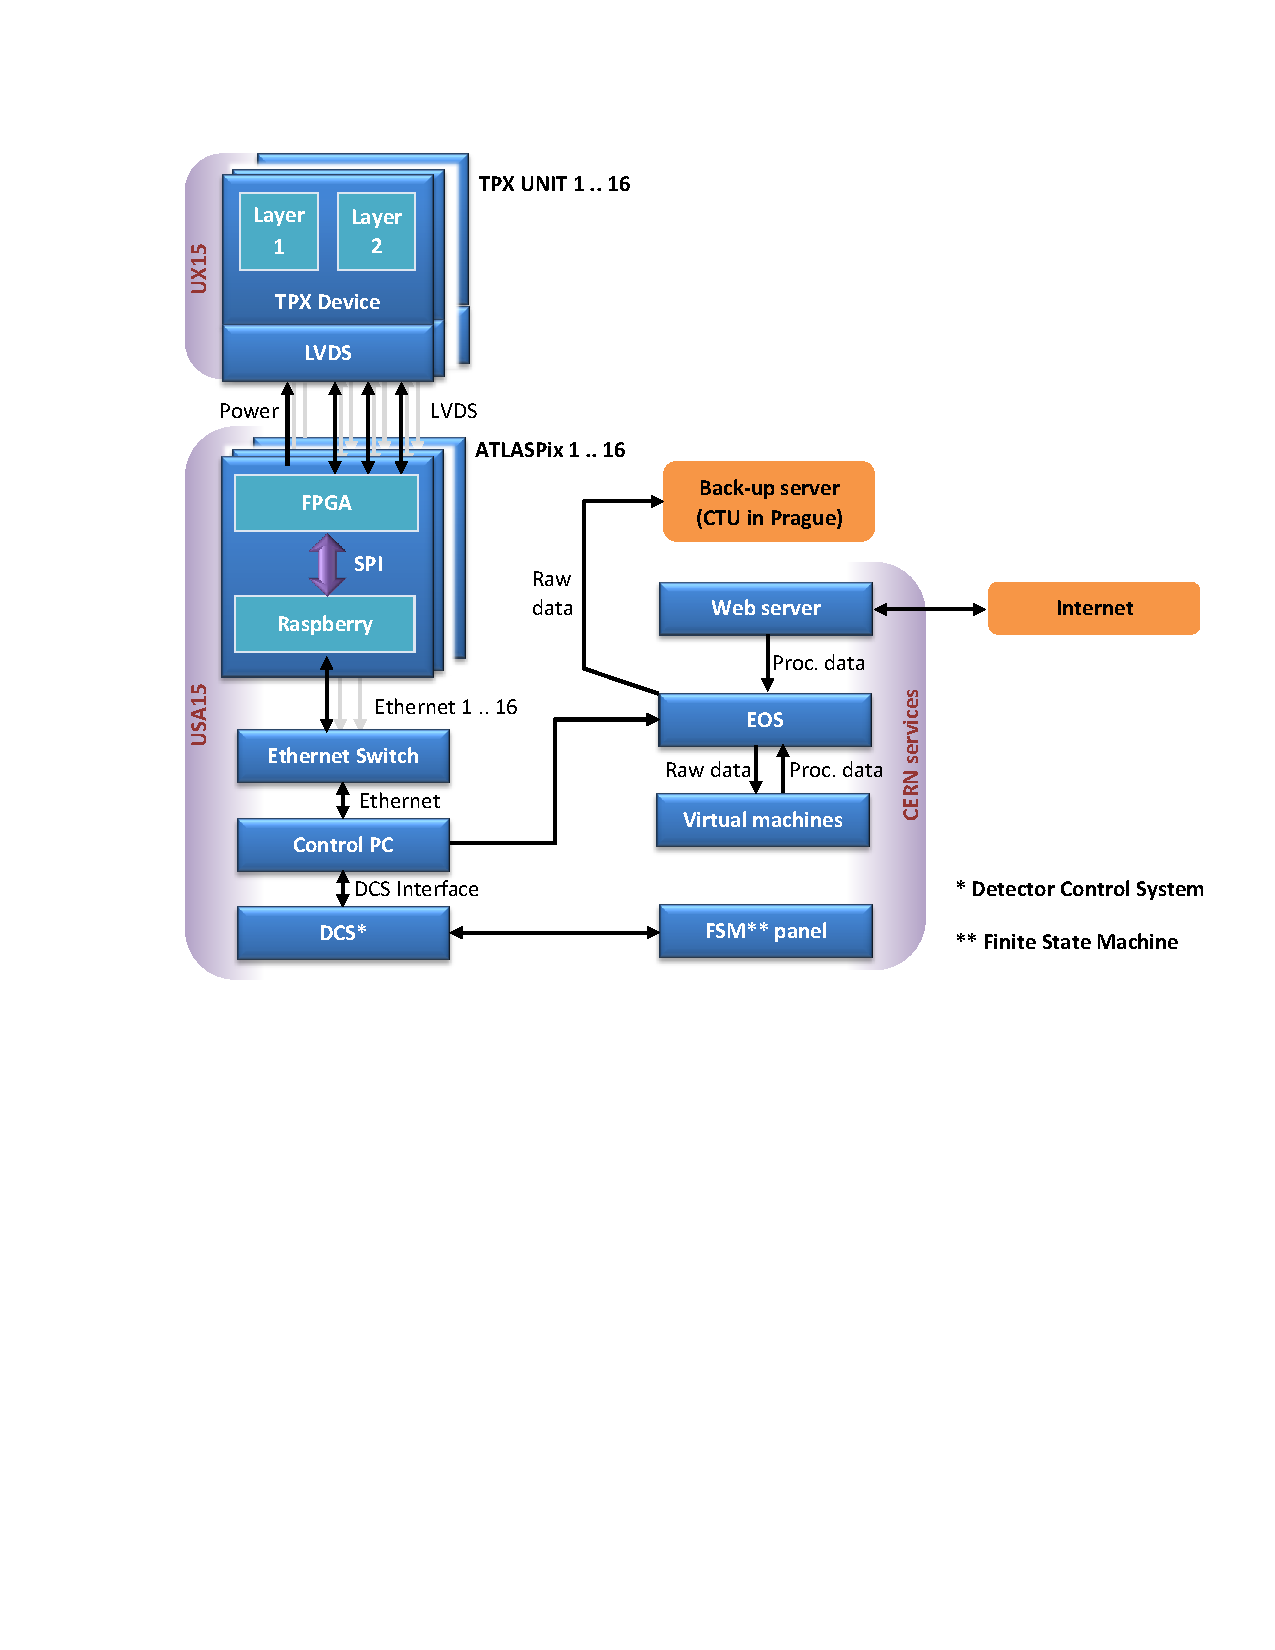
\includegraphics[clip, trim={2cm 11.2cm 0cm 2.6cm}, width=.5\textwidth, angle=0]{Plots/Doc1.pdf}
  \caption{Scheme of the readout, detector control, and data flow.}
  \label{fig:data_flow}
\end{figure}

Usually, frames taken by the TPX detectors are temporarily retained at the Control PC, then transferred to the EOS shared disk pool storage in 1-hour batches (see Fig.~\ref{fig:data_flow}). Once in EOS, data files become available to all users of the system. Due to high redundancy of the ASCII file format, data conversion is performed prior to any subsequent analysis. The conversion process is automatically scheduled as a job by the manager node after the data is confirmed to be valid and no detector malfunctions are suspected. In the course of this operation, frames are subject to cluster analysis~\cite{Holy2008} and measurements are combined with energy calibration data~\cite{Jakubek2011}. Results of this process are stored back in EOS in format compatible with the ROOT Data Analysis Framework~\cite{ROOT}.

The produced files are utilized as a database by the Data Visualization Application. Furthermore, these files serve as a starting point for further analysis performed manually. The original ASCII data files are compressed and downloaded to backup archive media.
